\section{Apéndice}

\begin{figure}[H]
    \centering
    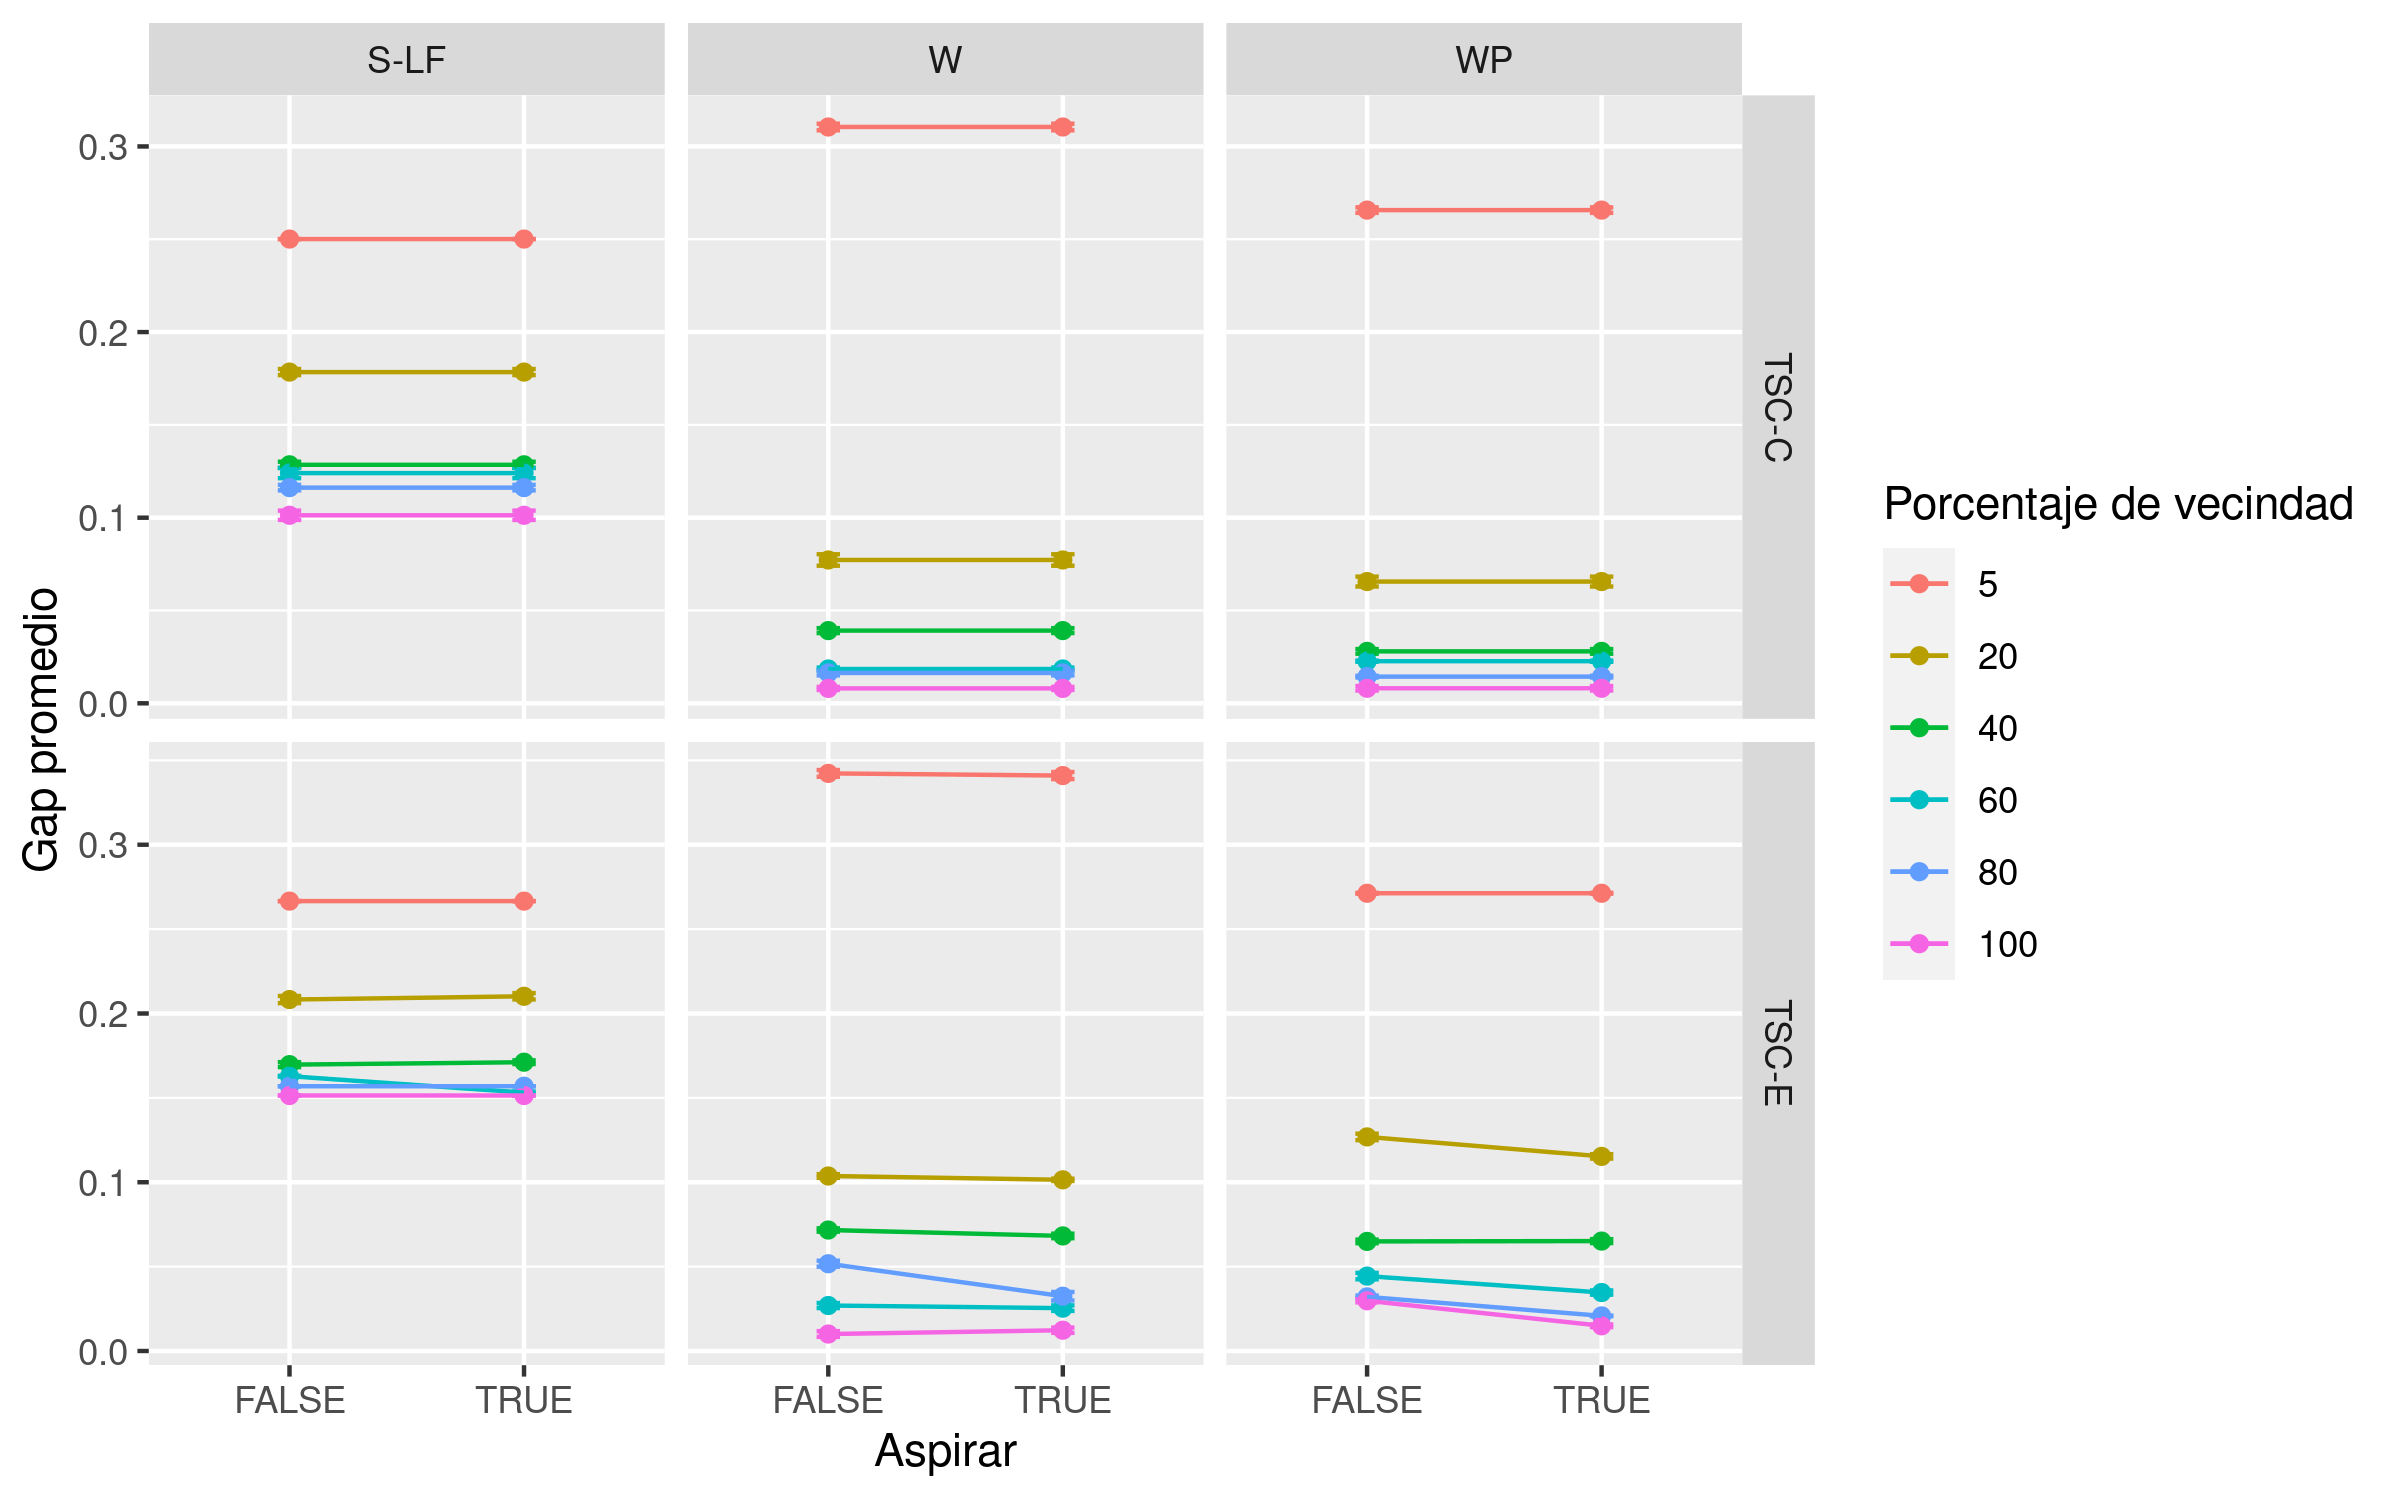
\includegraphics[scale = 0.7]{plots/suplementarias/aspirar_tsc.png}
    \caption{Gap relativo medio para ejecuciones de TSS activando o no la aspiración. Cada panel representa una combinación de heurística constructiva inicial y tipo de memoria. Los puntos representan el valor medio y las barras el error estándar. Se realizaron 5 repeticiones por instancia.}
    \label{plot:aspirar tsc}
\end{figure}

\begin{figure}[H]
    \centering
    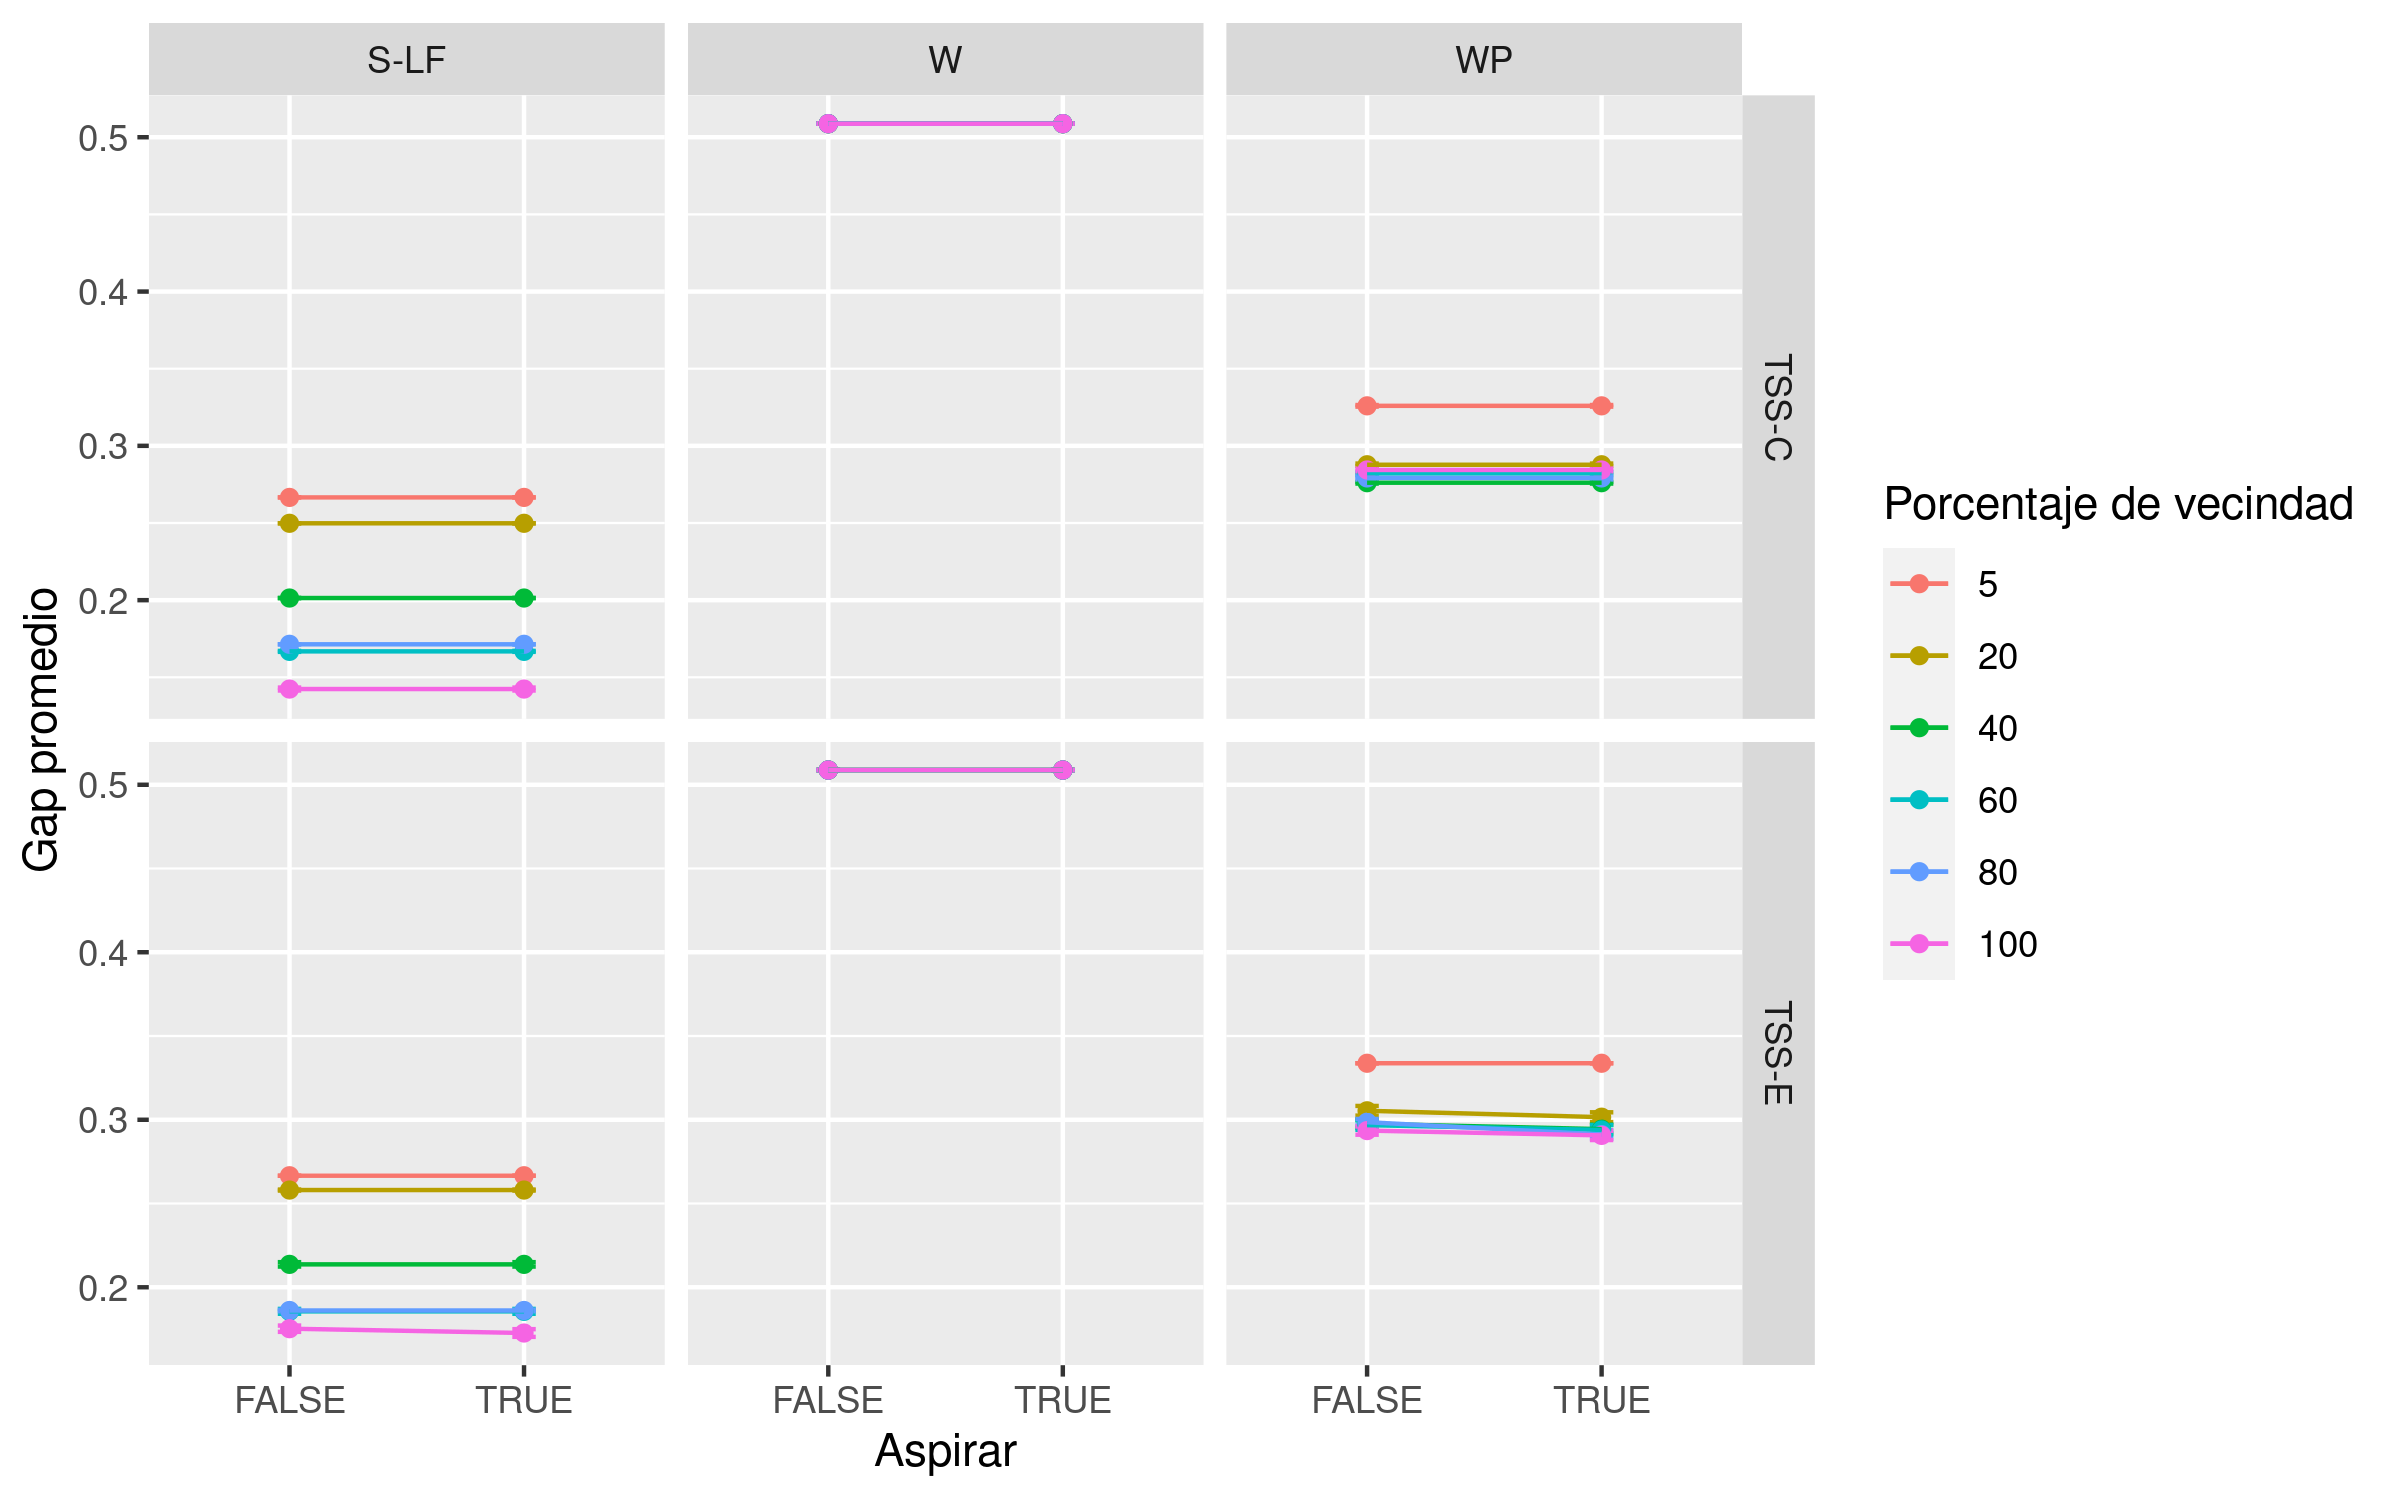
\includegraphics[scale = 0.7]{plots/suplementarias/aspirar_tss.png}
    \caption{Gap relativo medio para ejecuciones de TSS activando o no la aspiración. Cada panel representa una combinación de heurística constructiva inicial y tipo de memoria. Los puntos representan el valor medio y las barras el error estándar. Se realizaron 5 repeticiones por instancia.}
    \label{plot:aspirar tss}
\end{figure}


\begin{figure}[H]
    \centering
    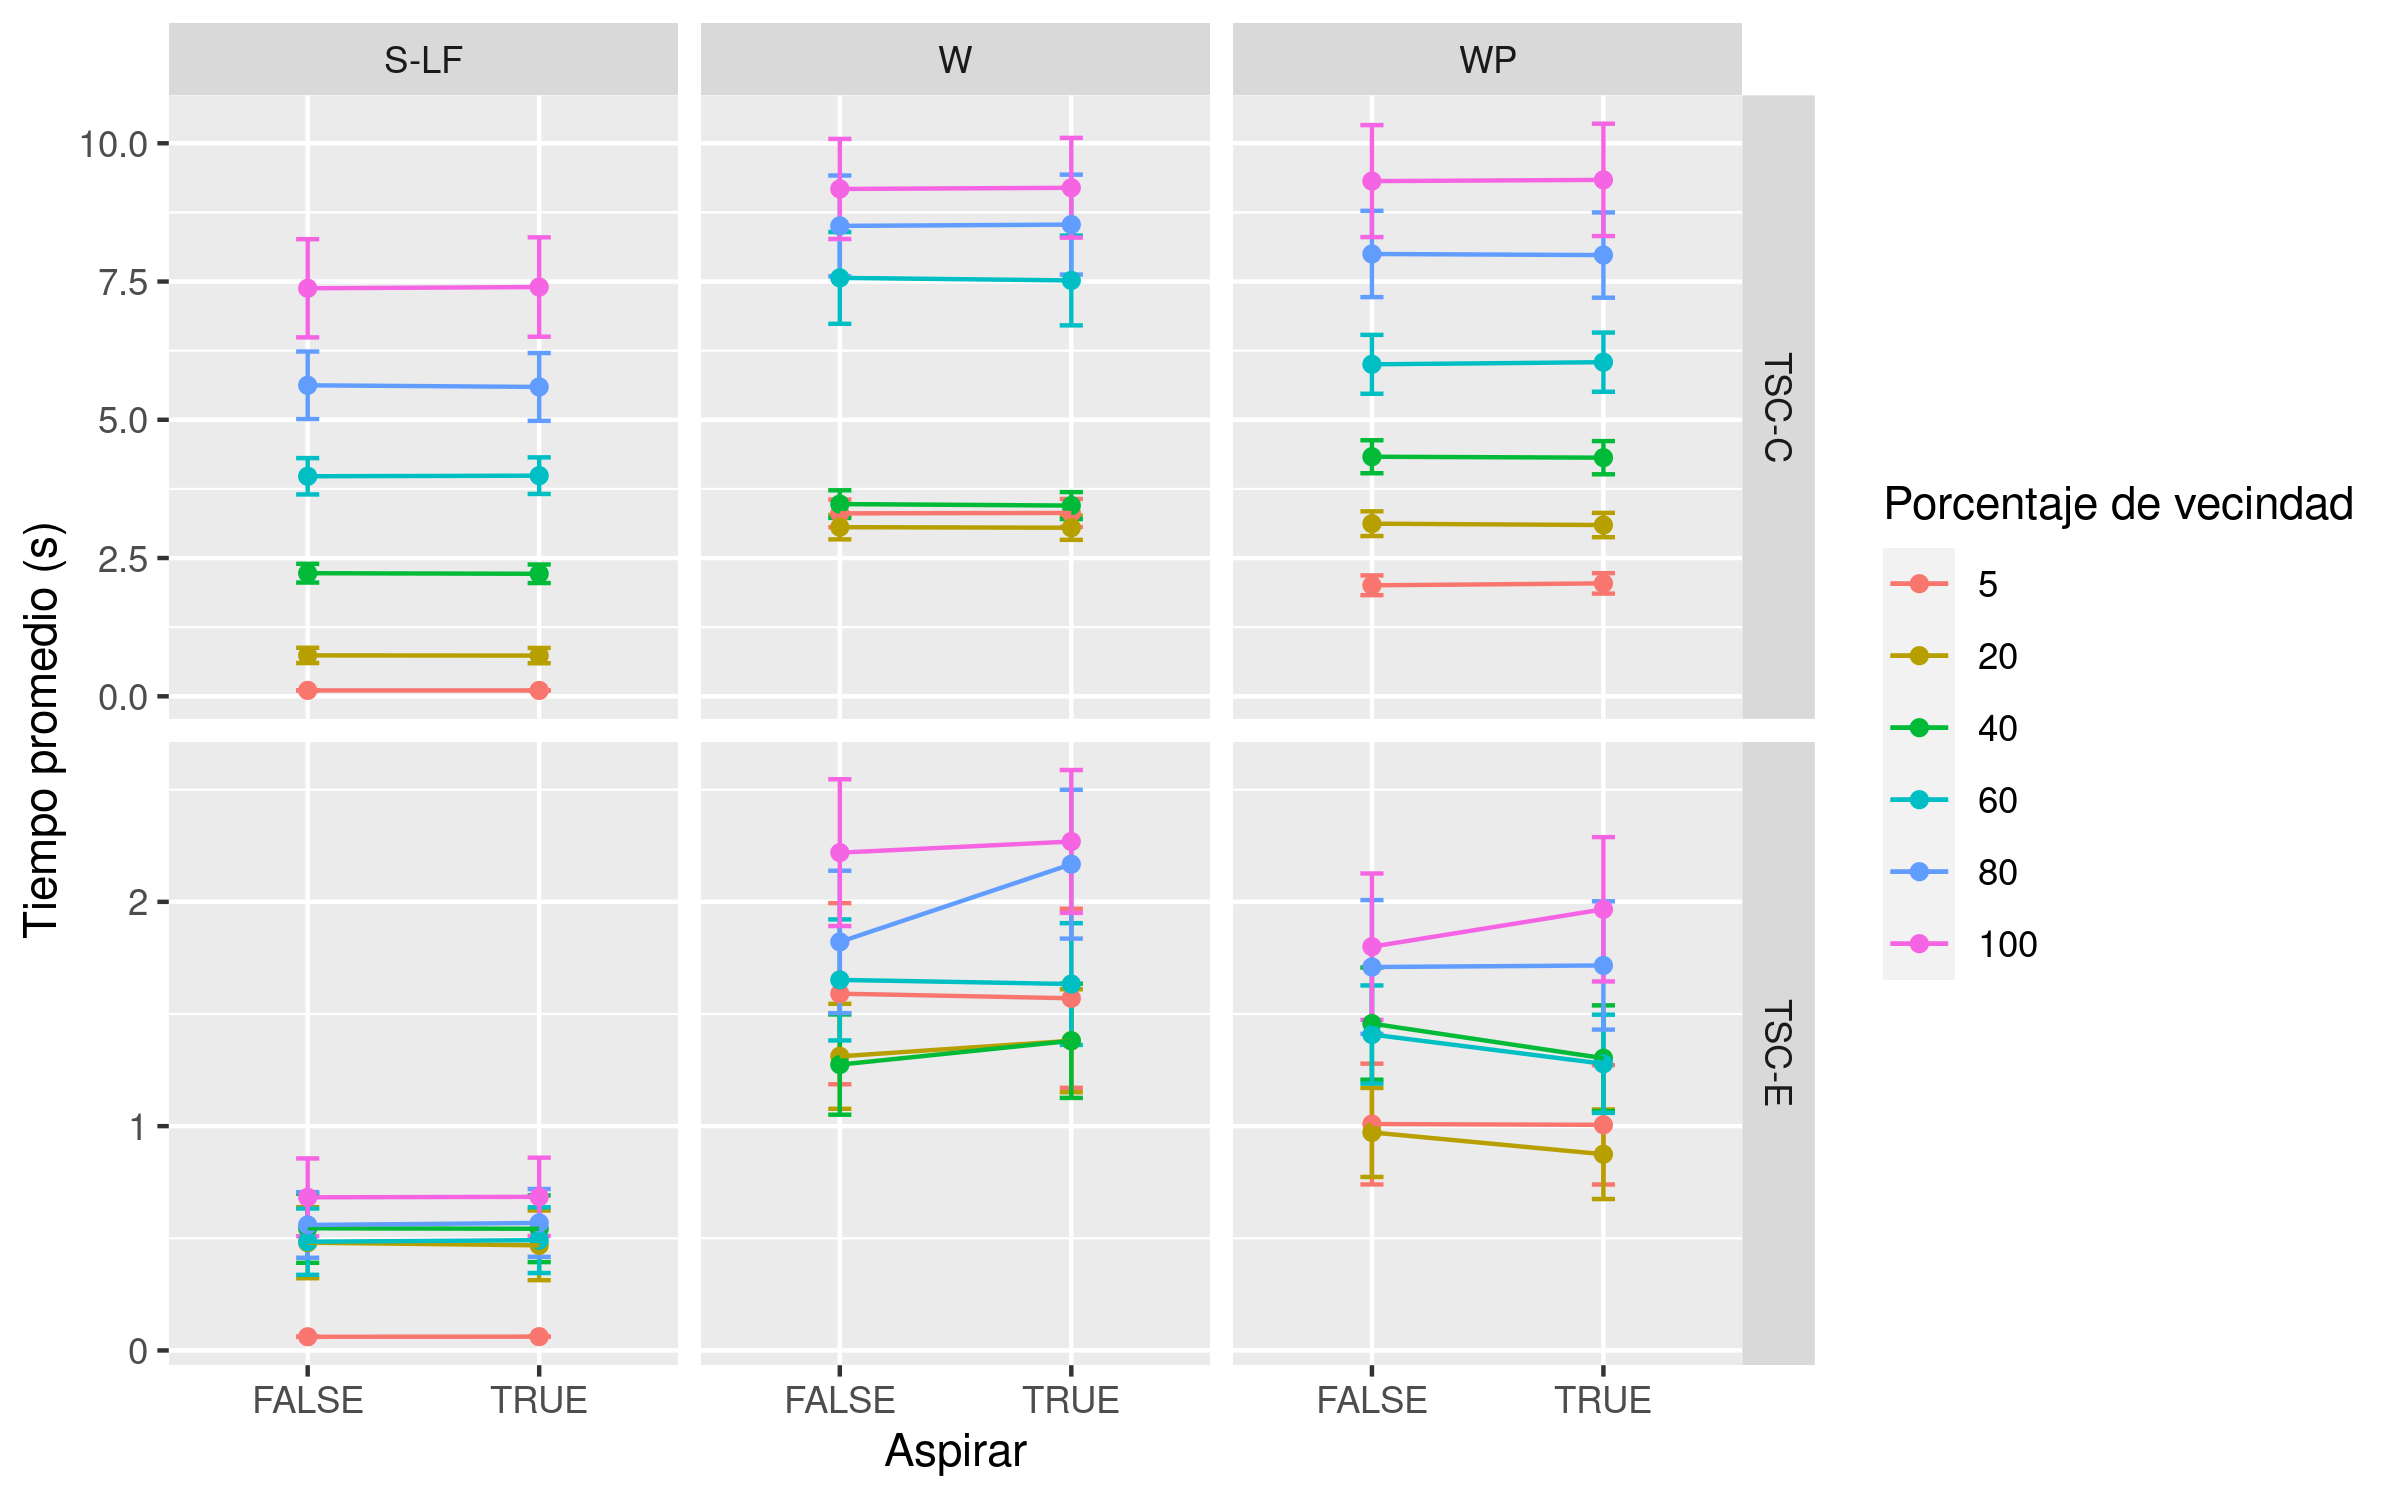
\includegraphics[scale = 0.7]{plots/suplementarias/aspirar_tiempo_tsc.png}
    \caption{Tiempo de ejecución medio para ejecuciones de TSC activando o no la aspiración. Cada panel representa una combinación de heurística constructiva inicial y tipo de memoria. Los puntos representan el valor medio y las barras el error estándar. Se realizaron 5 repeticiones por instancia.}
    \label{plot:aspirar tiempo tsc}
\end{figure}

\begin{figure}[H]
    \centering
    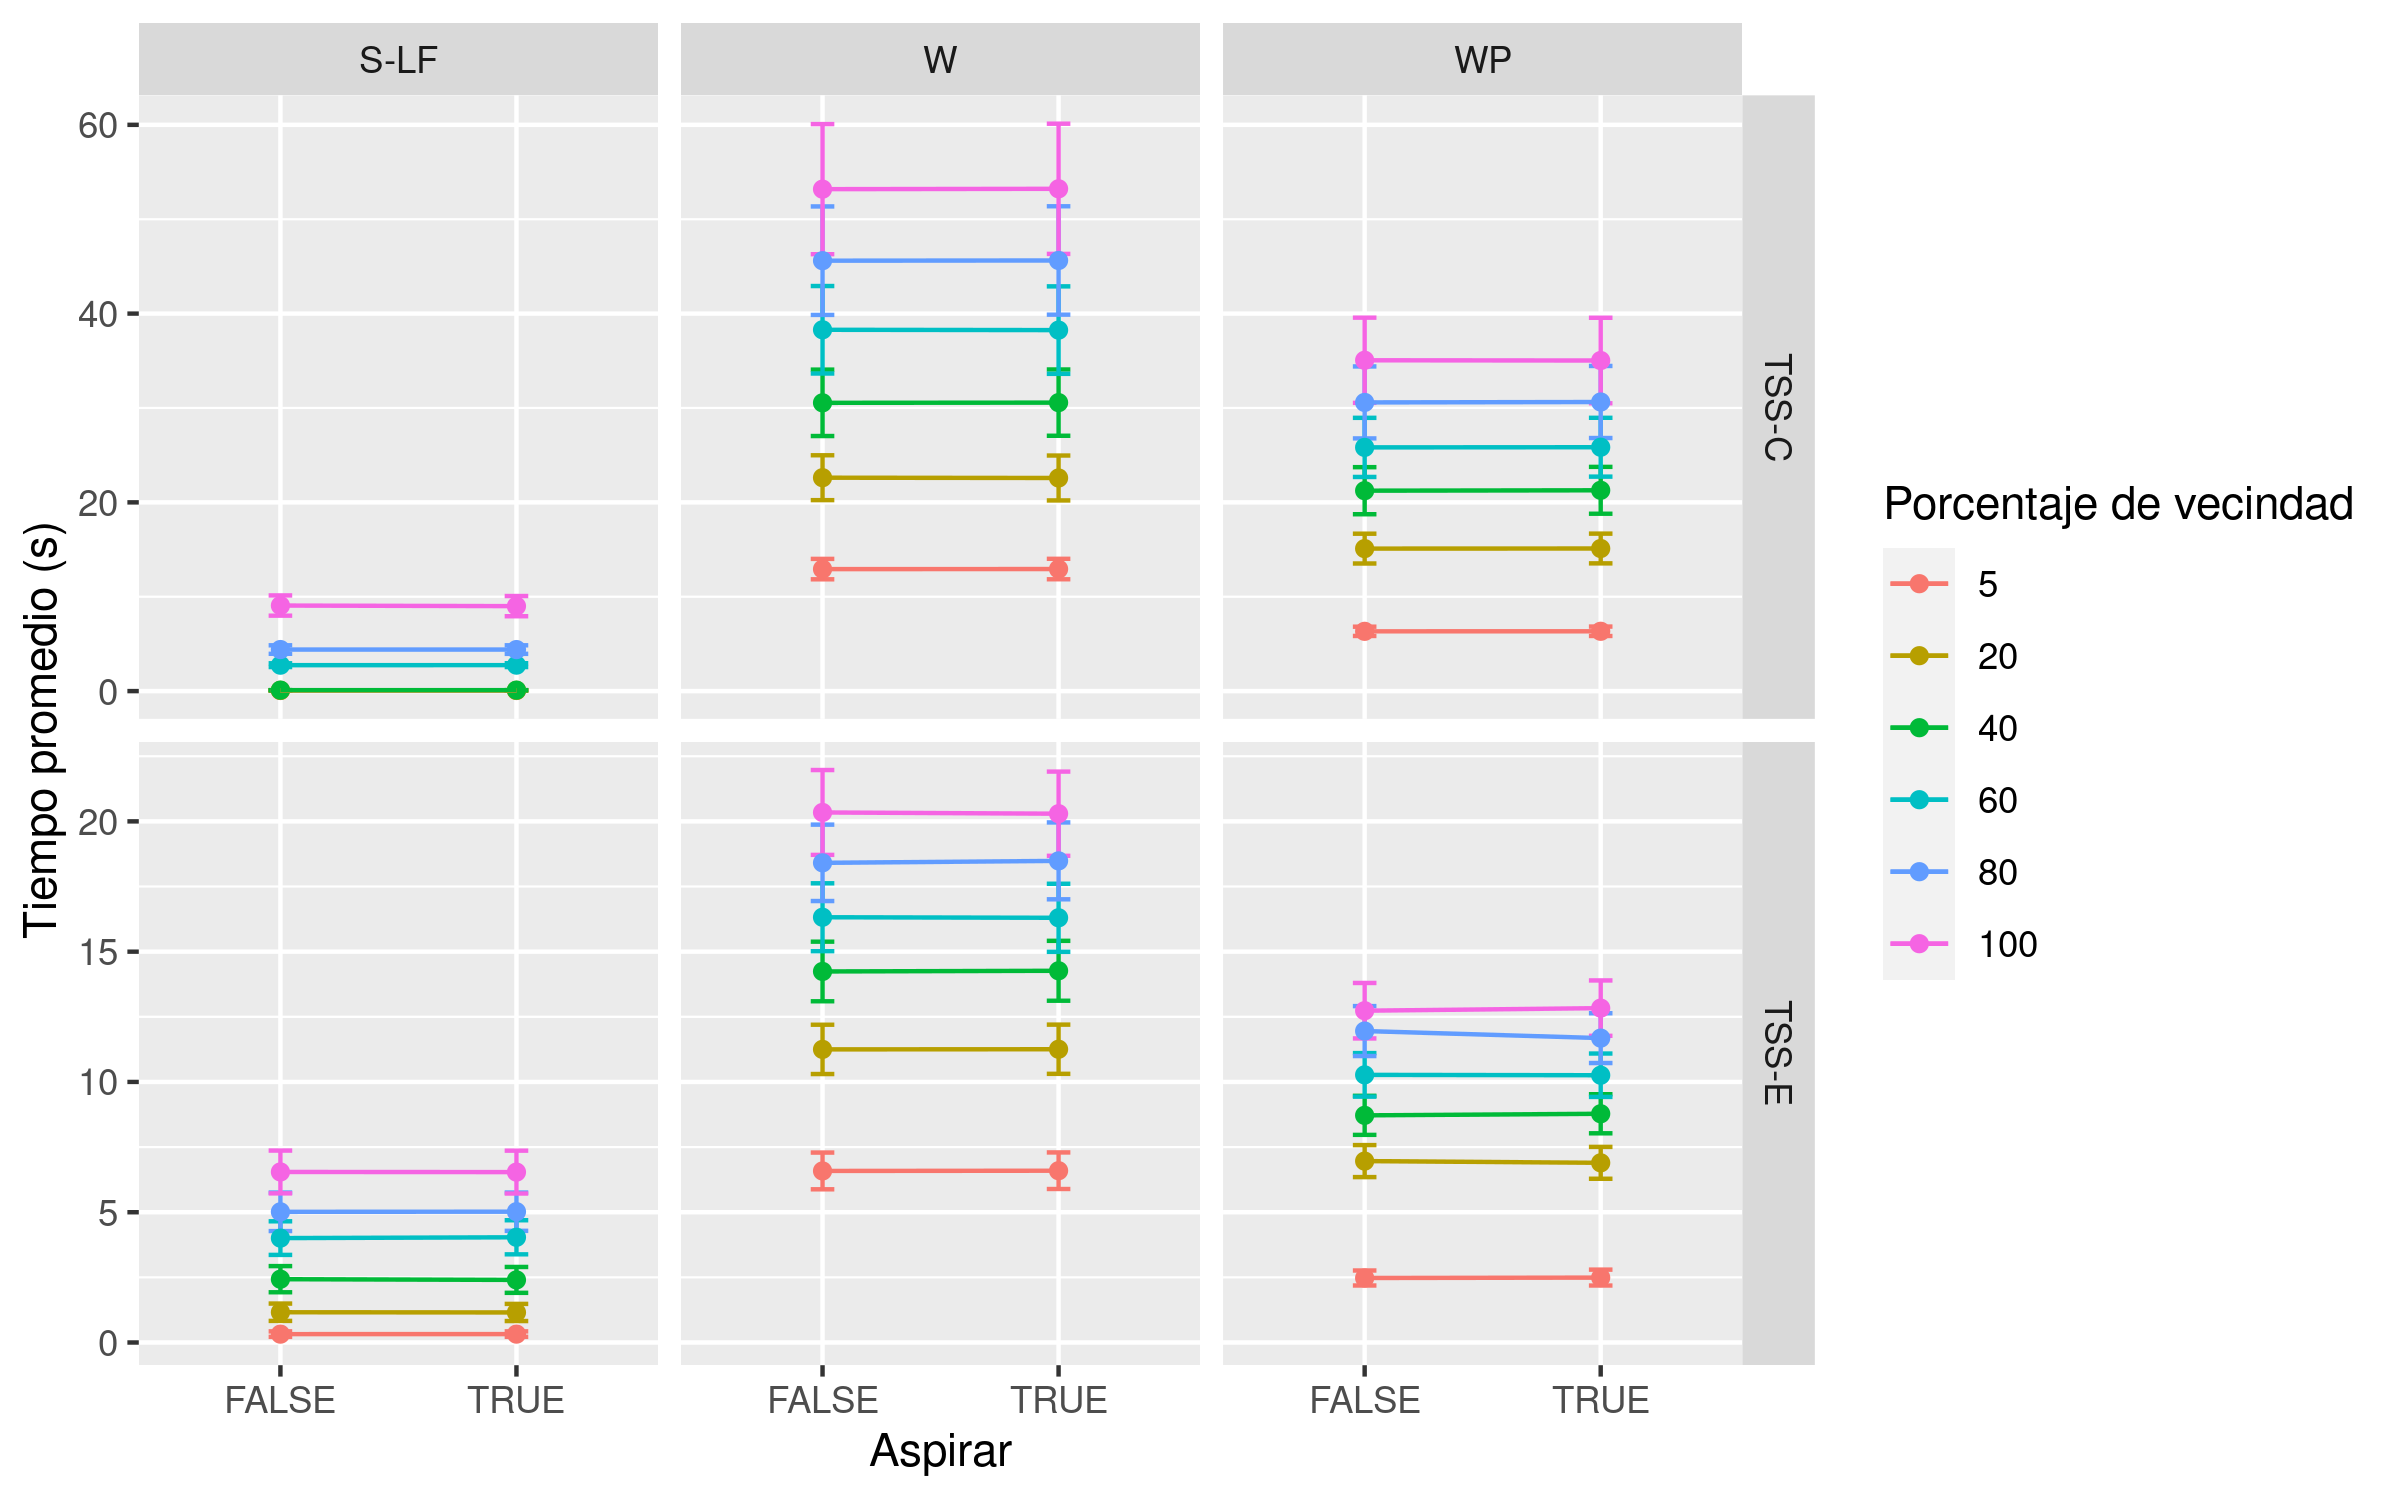
\includegraphics[scale = 0.7]{plots/suplementarias/aspirar_tiempo_tss.png}
    \caption{Tiempo de ejecución medio para ejecuciones de TSS activando o no la aspiración. Cada panel representa una combinación de heurística constructiva inicial y tipo de memoria. Los puntos representan el valor medio y las barras el error estándar. Se realizaron 5 repeticiones por instancia.}
    \label{plot:aspirar tiempo tss}
\end{figure}

\begin{figure}[H]
    \centering
    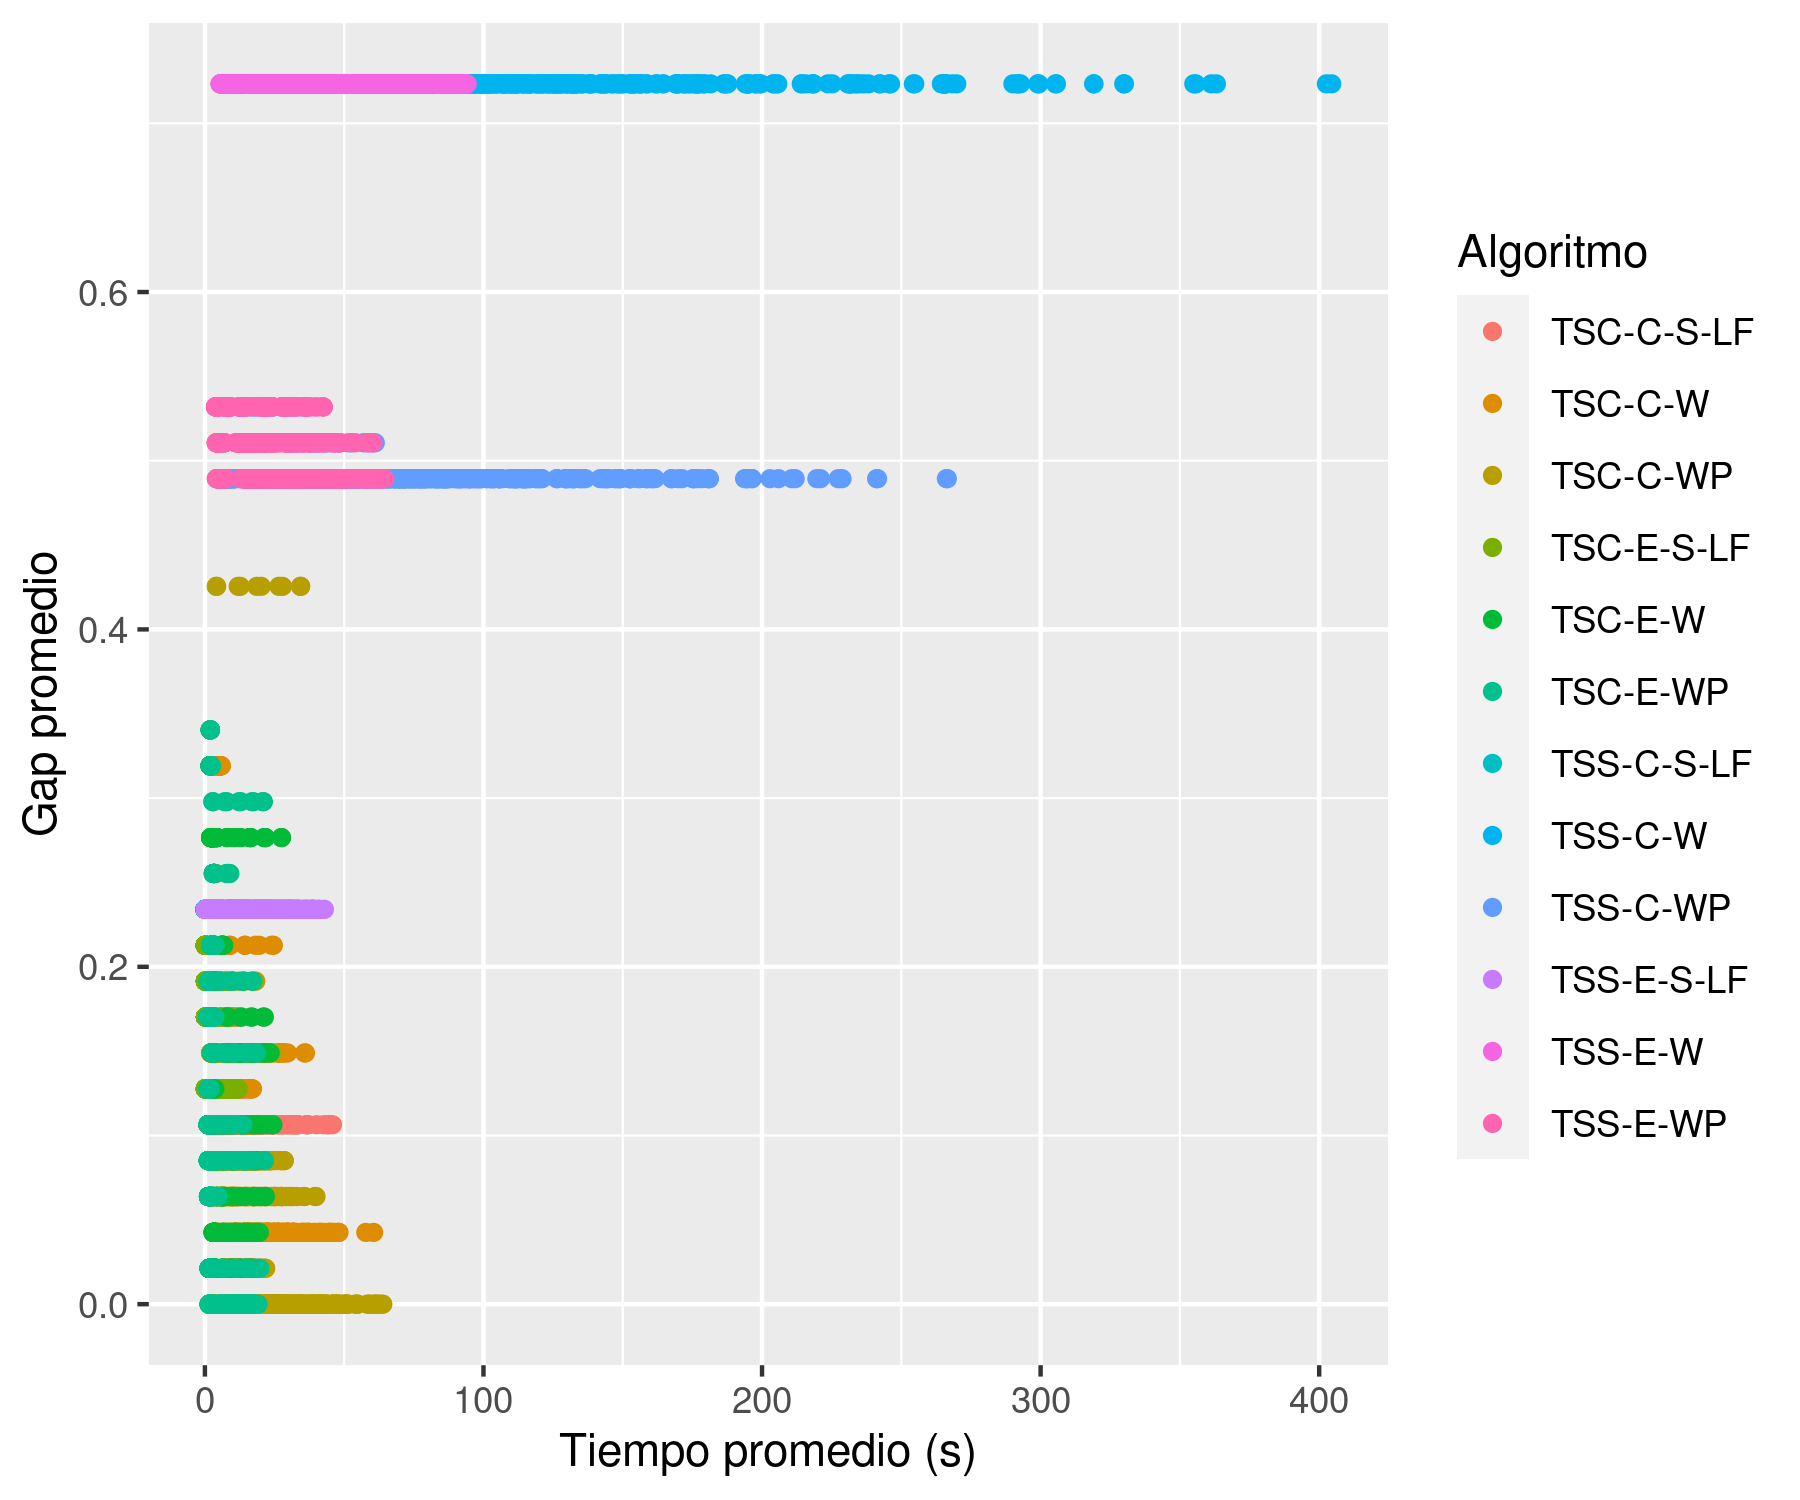
\includegraphics[scale = 0.7]{plots/suplementarias/gap_tiempo.png}
    \caption{Gap relativo promedio en función del tiempo promedio de ejecución. Los puntos representan el valor medio. Se realizaron 5 repeticiones por instancia. No se observa correlación.}
    \label{plot:correlacion gap tiempo}
\end{figure}